\begin{exercise}
      {ID-cf45d2a9ab3e30c9fab45c1425d2f313497c9861}
      {Klappleiter}
  \ifproblem\problem\par
    % <PROBLEM>
    Eine Klappleiter besitzt eine Länge von \SI{3}{\metre}.
    In welcher Höhe befindet sich das obere Lei\-ter\-en\-de,
    wenn die unteren Lei\-ter\-en\-den am Boden \SI{1.2}{\metre}
    weit auseinander stehen?
    % </PROBLEM>
  \fi
  %\ifoutline\outline\par
    % <OUTLINE>
    % </OUTLINE>
  %\fi
  \ifoutcome\outcome\par
    % <OUTCOME>
    Gesucht ist im Prinzip die Höhe eines
    gleichschenkligen Dreiecks
    mit den Seitenlängen \SI{3}{\metre},
    \SI{3}{\metre} und \SI{1.2}{\metre}:
    \begin{center}
      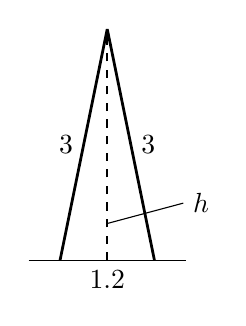
\begin{tikzpicture}
        % Leiter
        \draw[join=bevel, line width=1pt]
             (-0.6, 0     ) -- node[left]{\SI{3}{\metre}}
             ( 0.0, 2.9394) -- node[right]{\SI{3}{\metre}}
             ( 0.6, 0     );
        % Boden
        \draw[line width=0.6pt]
             (-1, 0) -- node[below]{\SI{1.2}{\metre}}
             ( 1, 0);
        % Hoehe
        \draw[style=dashed, line width=0.6pt]
             (0, 0) --
             (0, 2.9394);
        % Hilfslinie
        \draw (0, 0.47) -- ++(15:1cm) node[right] {$h$};
      \end{tikzpicture}
    \end{center}
    Da die Höhe $h$ senkrecht auf der Grundseite steht,
    gilt nach dem Satz des Pythagoras:
    \begin{equation*}
      h^2+\left(\frac{\SI{1.2}{\metre}}{2}\right)^2=3^2\text{\,\si{\square\metre}}
      \quad\Rightarrow\quad
      h^2+\SI{0.36}{\square\metre}=\SI{9}{\square\metre}
    \end{equation*}
    Wenn man diese Gleichung nach $h$ auflöst, erhält
    man die gesuchte Höhe:
    \begin{alignat*}{3}
      \relax&\quad
      &
      h^2+\SI{0.36}{\square\metre}&=\SI{9}{\square\metre}
      &
      \quad&|-\SI{0.36}{\square\metre}
      \\
      \Leftrightarrow&\quad
      &
      h^2&=\SI{8.64}{\square\metre}
      &
      \quad&|\,\sqrt{\ldots}
      \\
      \Leftrightarrow&\quad
      &
      h&\approx\SI{2.94}{\metre}
      &
      \quad&\relax
    \end{alignat*}
    Das obere Leiterende befindet sich also in
    einer Höhe von ca. \SI{2.94}{\metre}.
    % </OUTCOME>
  \fi
\end{exercise}
